The convergence of the proposed algorithms is demonstrated in this part. Figure \ref{fig:convergence} shows that the proposed
algorithms for both separated and shared deployments can converge in 10 iterations, which indicates the low complexity of the 
proposed algorithms.
\newpage

\begin{figure}[ht]
    \centering
    \subfigure[Algorithm for separated deployment]{
        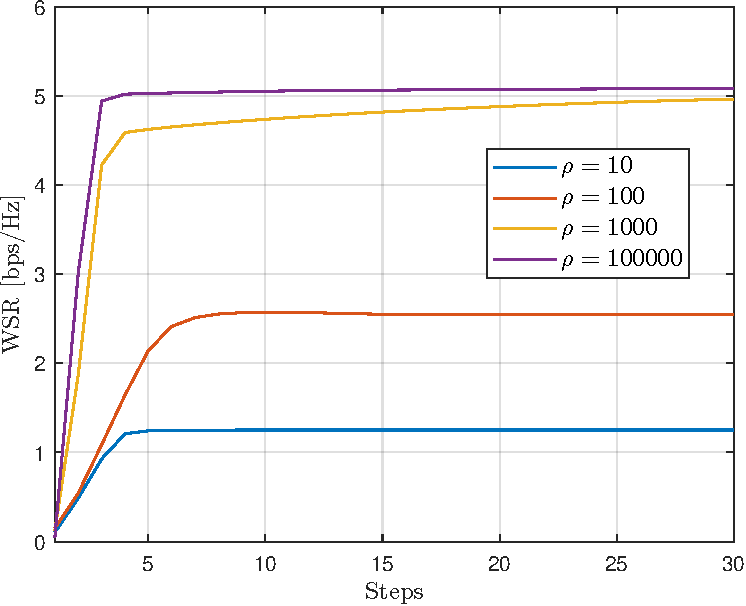
\includegraphics[width=0.475\textwidth]{convergence_separated.pdf}
        \label{fig:convergence_separated}
    }
    \subfigure[Algorithm for shared deployment]{
	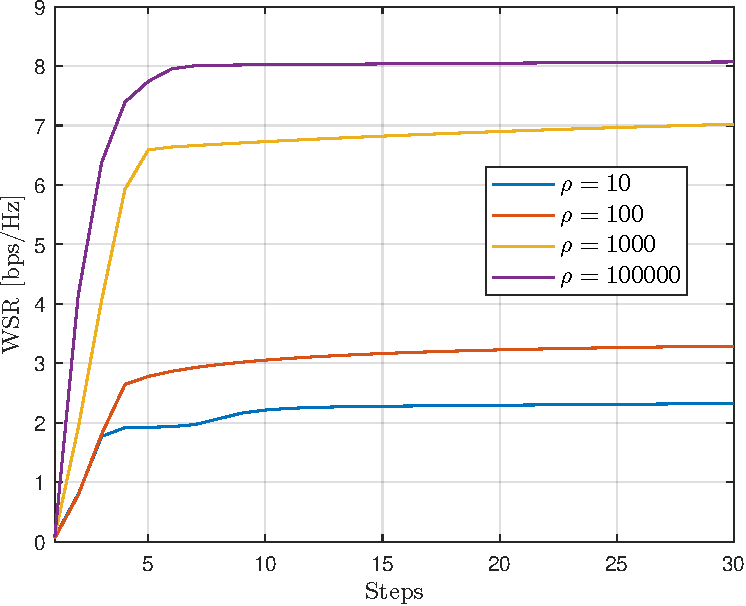
\includegraphics[width=0.475\textwidth]{convergence_shared.pdf}
        \label{fig:convergence_shared}
    }
    \caption{Convergence of proposed algorithms}
    \label{fig:convergence}
\end{figure}

Note that in Figure \ref{fig:convergence_shared}, the eigenvalue decomposition in used to approximate $\tilde{\bf p}_k^\star$ 
in SDR. In Figure \ref{fig:convergence_compare}, we compare the eigenvalue decomposition and Gaussian randomization in Algorithm \ref{alg:B}
when $\rho=100000$. It can be observed that the algorithm cannot converge when the Gaussian randomization is applied. 
The reason is that the $\tilde{\bf T}_k^\star$ calculated by CVX toolbox in practice is almost rank-one, i.e., the eigenvalues except
the largest one are almost zero. In this case, the Gaussian randomization cannot guarantee a good rank-one approximation.

\begin{figure}[ht]
    \centering
    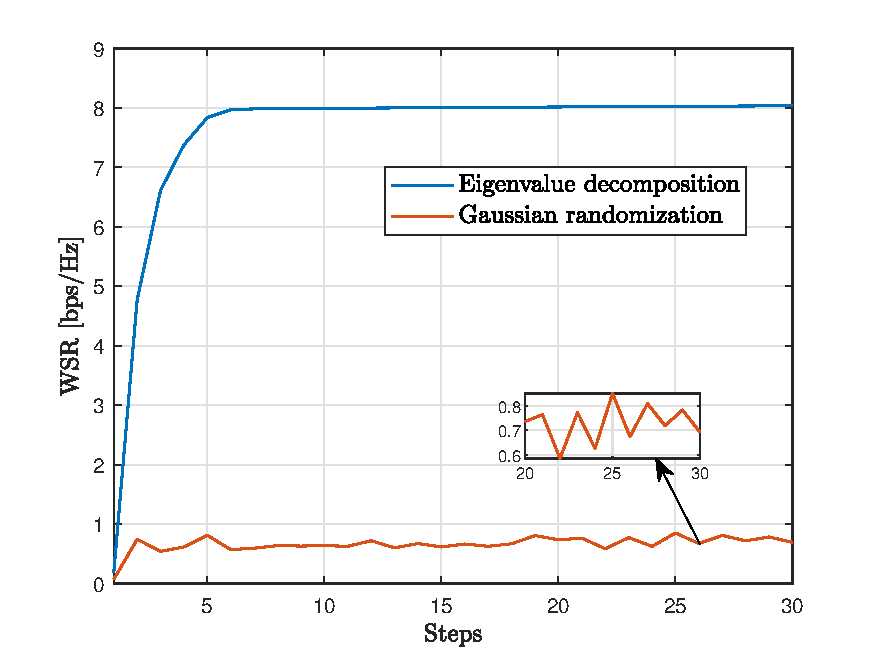
\includegraphics[width=0.6\textwidth]{convergence_shared_compare.pdf}
    \caption{Comparison of eigenvalue decomposition and Gaussian randomization}
    \label{fig:convergence_compare}
\end{figure}